% Documentation for pkuthss.
%
% Copyright (c) 2008-2009 solvethis
% Copyright (c) 2010-2016 Casper Ti. Vector
%
% This work may be distributed and/or modified under the conditions of the
% LaTeX Project Public License, either version 1.3 of this license or (at
% your option) any later version.
% The latest version of this license is in
%   https://www.latex-project.org/lppl.txt
% and version 1.3 or later is part of all distributions of LaTeX version
% 2005/12/01 or later.
%
% This work has the LPPL maintenance status `maintained'.
% The current maintainer of this work is Casper Ti. Vector.
%
% This work consists of the following files:
%   pkuthss.tex
%   chap/pkuthss-copyright.tex
%   chap/pkuthss-abstract.tex
%   chap/pkuthss-introduction.tex
%   chap/pkuthss-chap1.tex
%   chap/pkuthss-chap2.tex
%   chap/pkuthss-chap3.tex
%   chap/pkuthss-conclusion.tex
%   chap/pkuthss-encl1.tex
%   chap/pkuthss-acknowledge.tex

\documentclass[UTF8, openany]{pkuthss}
%新章开始(openright,openany):仅对book 文档类有效,默认值为openright,即每章都从奇数页开始;如果设置为openany,则每章仅从新的一页开始,不管奇偶页。

% \usepackage[
	% backend = biber, style = caspervector, utf8,
	% sorting = ecnty, giveninits = true, sortgiveninits = true
% ]{biblatex}
\usepackage{fancyvrb}
\usepackage{hologo}


\usepackage{float}
 %https://github.com/yihui/knitr/issues/1554   https://blog.csdn.net/littlefang/article/details/80110092
\usepackage{bicaption}
\captionsetup[figure][bi-first]{name=图}
\captionsetup[figure][bi-second]{name=Figure}

%\captionsetup[table][bi-first]{name=表}
%\captionsetup[table][bi-second]{name=Table}

% \setlength{\hfuzz}{3pt}
% \ctexset{linestretch = 2\ccwd}
% \setlength{\bibitemsep}{3bp}
% \renewcommand*{\bibfont}{\zihao{5}\linespread{1.27}\selectfont}

\hypersetup{colorlinks = true, allcolors = blue}
\newcommand{\myemph}[1]{\emph{\textcolor{red}{#1}}}
\newcommand{\unemph}[1]{\textup{\textcolor{black}{#1}}}
\newcommand{\docversion}{v1.7.4}

\pkuthssinfo{
	cthesisname = {博士学位论文}, ethesisname = {Undergraduate Thesis},
	ctitle = {厦门大学博士学位论文},
	etitle = {R bookdownplus},
	cauthor = {author},
	eauthor = {dapeng},
	studentid = {31415926},
	date = {2019-03-29},
	school = {R 语言学院},
	cmajor = {论文排版}, emajor = {Typesetting},
	direction = {bookdown},
	cmentor = {谷哥教授}, ementor = {Prof.Google},
	ckeywords = {排版,文档类},
	ekeywords = {\hologo{LaTeX2e}, \CTeX{}, bookdown}
}
% \addbibresource{pkuthss.bib}

%%%%%%%%%%%%%%
\usepackage{longtable,booktabs}

\usepackage{amssymb,amsmath}
\usepackage{natbib}
\bibliographystyle{apalike}
\newcommand{\VerbBar}{|}
\newcommand{\VERB}{\Verb[commandchars=\\\{\}]}
\DefineVerbatimEnvironment{Highlighting}{Verbatim}{commandchars=\\\{\}}
% Add ',fontsize=\small' for more characters per line
\usepackage{framed}
\definecolor{shadecolor}{RGB}{248,248,248}
\newenvironment{Shaded}{\begin{snugshade}}{\end{snugshade}}
\newcommand{\KeywordTok}[1]{\textcolor[rgb]{0.13,0.29,0.53}{\textbf{{#1}}}}
\newcommand{\DataTypeTok}[1]{\textcolor[rgb]{0.13,0.29,0.53}{{#1}}}
\newcommand{\DecValTok}[1]{\textcolor[rgb]{0.00,0.00,0.81}{{#1}}}
\newcommand{\BaseNTok}[1]{\textcolor[rgb]{0.00,0.00,0.81}{{#1}}}
\newcommand{\FloatTok}[1]{\textcolor[rgb]{0.00,0.00,0.81}{{#1}}}
\newcommand{\ConstantTok}[1]{\textcolor[rgb]{0.00,0.00,0.00}{{#1}}}
\newcommand{\CharTok}[1]{\textcolor[rgb]{0.31,0.60,0.02}{{#1}}}
\newcommand{\SpecialCharTok}[1]{\textcolor[rgb]{0.00,0.00,0.00}{{#1}}}
\newcommand{\StringTok}[1]{\textcolor[rgb]{0.31,0.60,0.02}{{#1}}}
\newcommand{\VerbatimStringTok}[1]{\textcolor[rgb]{0.31,0.60,0.02}{{#1}}}
\newcommand{\SpecialStringTok}[1]{\textcolor[rgb]{0.31,0.60,0.02}{{#1}}}
\newcommand{\ImportTok}[1]{{#1}}
\newcommand{\CommentTok}[1]{\textcolor[rgb]{0.56,0.35,0.01}{\textit{{#1}}}}
\newcommand{\DocumentationTok}[1]{\textcolor[rgb]{0.56,0.35,0.01}{\textbf{\textit{{#1}}}}}
\newcommand{\AnnotationTok}[1]{\textcolor[rgb]{0.56,0.35,0.01}{\textbf{\textit{{#1}}}}}
\newcommand{\CommentVarTok}[1]{\textcolor[rgb]{0.56,0.35,0.01}{\textbf{\textit{{#1}}}}}
\newcommand{\OtherTok}[1]{\textcolor[rgb]{0.56,0.35,0.01}{{#1}}}
\newcommand{\FunctionTok}[1]{\textcolor[rgb]{0.00,0.00,0.00}{{#1}}}
\newcommand{\VariableTok}[1]{\textcolor[rgb]{0.00,0.00,0.00}{{#1}}}
\newcommand{\ControlFlowTok}[1]{\textcolor[rgb]{0.13,0.29,0.53}{\textbf{{#1}}}}
\newcommand{\OperatorTok}[1]{\textcolor[rgb]{0.81,0.36,0.00}{\textbf{{#1}}}}
\newcommand{\BuiltInTok}[1]{{#1}}
\newcommand{\ExtensionTok}[1]{{#1}}
\newcommand{\PreprocessorTok}[1]{\textcolor[rgb]{0.56,0.35,0.01}{\textit{{#1}}}}
\newcommand{\AttributeTok}[1]{\textcolor[rgb]{0.77,0.63,0.00}{{#1}}}
\newcommand{\RegionMarkerTok}[1]{{#1}}
\newcommand{\InformationTok}[1]{\textcolor[rgb]{0.56,0.35,0.01}{\textbf{\textit{{#1}}}}}
\newcommand{\WarningTok}[1]{\textcolor[rgb]{0.56,0.35,0.01}{\textbf{\textit{{#1}}}}}
\newcommand{\AlertTok}[1]{\textcolor[rgb]{0.94,0.16,0.16}{{#1}}}
\newcommand{\ErrorTok}[1]{\textcolor[rgb]{0.64,0.00,0.00}{\textbf{{#1}}}}
\newcommand{\NormalTok}[1]{{#1}}
%%%%%%%%%%%%%%

\begin{document}

\frontmatter
%\maketitle
\pagestyle{empty}
\setcounter{page}{0}
\pagenumbering{Roman}

\begin{cabstract}

%	这里写中文摘要。啊不可挡家真的好。
这里写中文摘要。啊不可挡家真的好。
	
\end{cabstract}

\cleardoublepage

\begin{eabstract}

%	Abstract in English. R bookdownplus is amazing.
Abstract in English. R bookdownplus is amazing.

\end{eabstract}

\cleardoublepage

\pagestyle{plain}

\tableofcontents

\cleardoublepage

\mainmatter

\hypertarget{test}{%
\chapter*{Test}\label{test}}
\addcontentsline{toc}{chapter}{Test}

\markboth{test}{}

\begin{figure}
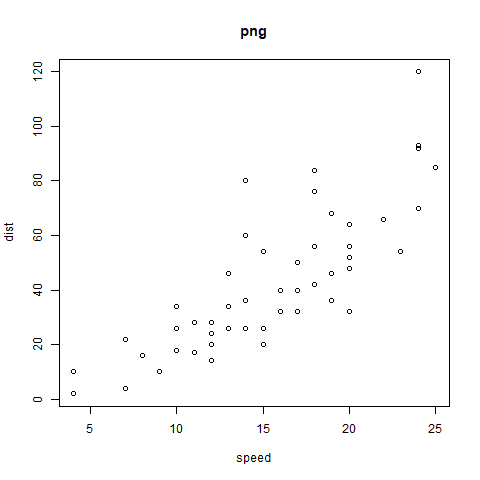
\includegraphics{figures/fig} \caption[bla]{bla}\label{fig:gb}
\end{figure}

\begin{Shaded}
\begin{Highlighting}[]
\NormalTok{knitr}\OperatorTok{::}\KeywordTok{include_graphics}\NormalTok{(}\StringTok{"figures/fig.png"}\NormalTok{)}
\end{Highlighting}
\end{Shaded}

\begin{figure}[!htp]

\begin{center}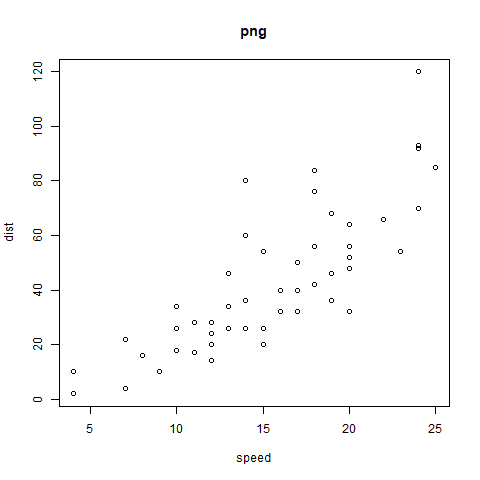
\includegraphics[width=0.328\linewidth]{figures/fig} \end{center}

\bicaption{上海交通大学}{SJTU}\end{figure}

\begin{Shaded}
\begin{Highlighting}[]
\NormalTok{bookdown}\OperatorTok{::}\KeywordTok{preview_chapter}\NormalTok{(}\StringTok{"00-preface.Rmd"}\NormalTok{, }
  \DataTypeTok{output_format=}\StringTok{"bookdown::gitbook"}\NormalTok{, }\DataTypeTok{encoding=}\StringTok{"UTF-8"}\NormalTok{)}
\end{Highlighting}
\end{Shaded}

\cleardoublepage

\mainmatter

\hypertarget{chap0}{%
\chapter{绪论}\label{chap0}}

The eukaryotes (0.8--3 µm) are a taxonomically diverse group that includes representatives from four algal phyla: the Chlorophyta, Haptophyta, Cryptophyta and Heterokontophyta (Vaulot et al., 2008).\citep{buitenhuis2012picophytoplankton}

很高兴地宣布,我的 R 语言扩展包 `bookdownplus' \citep{R-bookdownplus} 在 CRAN 正式发布了。

bookdownplus 是对 bookdown 包 \citep{R-bookdown} 的增强和简化。bookdown 就好比 Microsoft Word 或 LaTeX,可以用来写文档,而 bookdownplus 提供了很多有用的模板,可以很方便地在 bookdown 平台写期刊论文、学位论文、学术海报、化学分子式、信件、日记、日历、诗集、吉他谱等各种常用文档和书籍。这是功能上的增强(+)。

bookdownplus 使用时只需指定一个模板,给定作者和书名,就可以一键生成模板文件,用户在模板文件里照猫画虎写自己的文字就可以了,不必再花力气上网找模板、设置 YAML 和 LaTeX。这是操作上的简化(-)。

bookdownplus 各个模板的使用方法详见 \href{https://bookdown.org/baydap/bookdownplus}{R bookdownplus Textbook}。这本电子书本身就是用 bookdownplus 生成的,尤其是它的 \href{https://bookdown.org/baydap/bookdownplus/bookdownplus.pdf}{pdf 版本}很美观。此书的源码开放,可以作为使用 bookdownplus写书的示例。

\begin{figure}[H]

{\centering 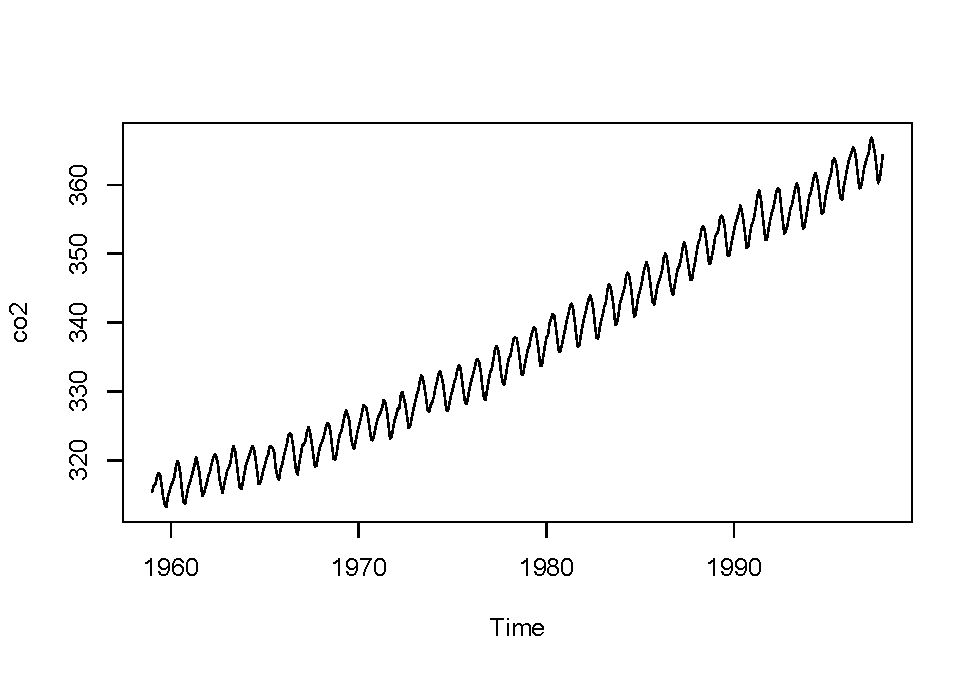
\includegraphics[width=0.8\linewidth]{xmu_phd_files/figure-latex/co2-1} 

}

\caption[用 R 语言画个图试试]{用 R 语言画个图试试}\label{fig:co2}
\end{figure}

图 \ref{fig:co2} 是 CO\textsubscript{2} 数据。

表 \ref{tab:tabair} 是空气质量数据。

\begin{Shaded}
\begin{Highlighting}[]
\NormalTok{knitr}\OperatorTok{::}\KeywordTok{kable}\NormalTok{(}\KeywordTok{head}\NormalTok{(airquality), }\DataTypeTok{caption =} \StringTok{'空气质量数据。'}\NormalTok{,}
                   \DataTypeTok{booktabs =} \OtherTok{TRUE}\NormalTok{)}
\end{Highlighting}
\end{Shaded}

\begin{table}[t]

\caption{\label{tab:tabair}空气质量数据。}
\centering
\begin{tabular}{rrrrrr}
\toprule
Ozone & Solar.R & Wind & Temp & Month & Day\\
\midrule
41 & 190 & 7.4 & 67 & 5 & 1\\
36 & 118 & 8.0 & 72 & 5 & 2\\
12 & 149 & 12.6 & 74 & 5 & 3\\
18 & 313 & 11.5 & 62 & 5 & 4\\
NA & NA & 14.3 & 56 & 5 & 5\\
\addlinespace
28 & NA & 14.9 & 66 & 5 & 6\\
\bottomrule
\end{tabular}
\end{table}

表 \ref{tab:md} 是常用 markdown 语法。

\begin{longtable}[]{@{}lr@{}}
\caption{\label{tab:md} Markdown 语法}\tabularnewline
\toprule
标记示例 & 输出\tabularnewline
\midrule
\endfirsthead
\toprule
标记示例 & 输出\tabularnewline
\midrule
\endhead
\texttt{*italic*} & 斜体 \emph{italic}\tabularnewline
\texttt{**粗体**} & \textbf{粗体}\tabularnewline
\texttt{CO\textasciitilde{}2\textasciitilde{}} & 下标(CO\textsubscript{2})\tabularnewline
\texttt{R\^{}2\^{}} & 上标(R\textsuperscript{2})\tabularnewline
\texttt{{[}网站{]}(http://xuer.pzhao.net)} & 超级链接\href{http://xuer.pzhao.net}{网站}\tabularnewline
\texttt{\textless{}xuer@pzhao.net\textgreater{}} & 邮件链接 \href{mailto:xuer@pzhao.net}{\nolinkurl{xuer@pzhao.net}}\tabularnewline
\texttt{!{[}{]}(http图片链接)} & 插入图片\tabularnewline
\texttt{\textgreater{}\ 引用文字} & 引用\tabularnewline
\texttt{\textasciigrave{}plot()\textasciigrave{}} & 行间代码\tabularnewline
四个空格 & 整行代码\tabularnewline
三个反引号 & 区块代码\tabularnewline
\texttt{\#\ 第一章} & 章节标题\tabularnewline
\texttt{1.\ 列表...} & 带编号的列表\tabularnewline
\texttt{-\ 列表...} & 不带编号的列表\tabularnewline
\texttt{\^{}{[}脚注{]}} & 脚注\footnote{脚注}\tabularnewline
\bottomrule
\end{longtable}

材料与方法

\hypertarget{section}{%
\section{准备}\label{section}}

在开始前,需要安装 R, RStudio, bookdown,和其他依赖的软件和包(例如 \texttt{Pandoc}, LaTeX, \texttt{rmarkdown}, \texttt{rticle}, \texttt{knitr}等),作为准备。详见 \href{https://bookdown.org/yihui/bookdown/}{bookdown 官方手册}。

\hypertarget{section-1}{%
\section{安装}\label{section-1}}

准备完毕后,就可以安装 bookdownplus 了。可以安装稳定版:

\begin{verbatim}
install.packages("bookdownplus")
\end{verbatim}

或开发版:

\begin{verbatim}
devtools::install_github("pzhaonet/bookdownplus")
\end{verbatim}

\hypertarget{section-2}{%
\section{生成模板文件}\label{section-2}}

接着,在 R 中运行下面的代码:

\begin{verbatim}
bookdownplus::bookdownplus()
\end{verbatim}

这时,在你的工作目录(\texttt{getwd()}),会得到一些模板文件(如 \texttt{index.Rmd},\texttt{body.Rmd}, \texttt{bookdownplus.Rproj}) 和文件夹。

\hypertarget{section-3}{%
\section{编译成书}\label{section-3}}

用 RStudio 打开 \texttt{bookdownplus.Rproj}文件,然后按 \texttt{ctrl+shift+b},Duang!你就得到模板书 \texttt{*.pdf}了!保存在 \texttt{\_book/} 文件夹里。

\hypertarget{section-4}{%
\section{你的文字}\label{section-4}}

在 \texttt{index.Rmd} 和 \texttt{body.Rmd} 里写你自己的文字,享受写书的快乐吧!自古皆死,不朽者文。

\hypertarget{section-5}{%
\section{更多输出格式}\label{section-5}}

模板默认生成的书是pdf格式。`bookdownplus' 从 1.0.3 开始,可以很方便地输出更多格式,包括国内最常见的 'word'格式,网页'html'格式和电子书'epub'格式,只需运行:

\begin{Shaded}
\begin{Highlighting}[]
\NormalTok{bookdownplus}\OperatorTok{::}\KeywordTok{bookdownplus}\NormalTok{(}\DataTypeTok{template =} \StringTok{'article'}\NormalTok{, }
    \DataTypeTok{more_output =} \KeywordTok{c}\NormalTok{(}\StringTok{'html'}\NormalTok{, }\StringTok{'word'}\NormalTok{, }\StringTok{'epub'}\NormalTok{))}
\end{Highlighting}
\end{Shaded}

就可以在 \texttt{\_book/} 文件夹里看到这些文件了。

网页格式可以极其方便地免费发布到 \href{https://bookdown.org}{bookdown.org},只需运行:

\begin{verbatim}
bookdown::publish_book()
\end{verbatim}

这里是 bookdown 书籍的大本营。

\hypertarget{section-6}{%
\section{更多建议}\label{section-6}}

我开发的另外两个 R 包可以配合 `bookdown' 使用:

\begin{itemize}
\item
  mindr,可以从 markdown 或 R markdown 格式的书稿中提取纲要,并且生成思维导图。
\item
  pinyin,可以为书稿的章节标题自动生成\href{https://bookdown.org/yihui/bookdown/cross-references.html}{`\{\#ID\}'}。如果标题里含有汉字,就会自动转换成拼音。
\end{itemize}

具体用法见他们的帮助信息。这两个包已经在 CRAN正式发布,安装命令是:

\begin{verbatim}
install.packages('mindr')
install.packages('pinyin')`.
\end{verbatim}

\hypertarget{chap2}{%
\chapter{南海东北部微型鞭毛虫对异养细菌摄食速率之日变动规律}\label{chap2}}

1111111

\appendix

\bibliography{config/bib}

\hypertarget{section-7}{%
\chapter{定理推倒}\label{section-7}}

\raggedbottom

\hypertarget{a-}{%
\section{定理 A 的推倒}\label{a-}}

\flushbottom

\backmatter

\hypertarget{section-8}{%
\chapter{致谢}\label{section-8}}

本模板源自 Casper Ti. Vector 的 \LaTeX\{\} 模板\footnote{\url{https://gitlab.com/CasperVector/pkuthss}}。

感谢中国海洋研究超级QQ群(183403725)各位群友在知识交流上的帮助。

\end{document}
